\subsection{Gesamtsystem}
Das Gesamtsystem wurde so g\"unstig wie m\"oglich aufgebaut. Wenn die einelnen Komponenten bei den Preiswertesten Lieferanten bezogen werden, dann kann das gesamte Ger\"at unter 150CHF (exkl. Geh\"ause) erstellt werden. Die Nachfolgende Tabelle (\tref{tKosten}) zeigt eine Auflistung der Kosten des Geräts.

\begin{table}[H]
\centering
    \begin{tabular}{ll}
    \textbf{Komponente}                & \textbf{Preis}   \\
    NanoPi NEO                         & 10 CHF  \\
    Full HD Kamera                     & 50 CHF  \\
    Autobatterie                       & 50 CHF  \\ 
    WIFI-Adapter                       & 10 CHF  \\
    USB-Hub                            & 5 CHF   \\
    Spannungswandler                   & 10 CHF  \\
    Kleinteile (Schrauben, Kabel, usw) & 15 CHF  \\ \hline
    \textbf{Gesamt}                    & \textbf{150 CHF} \\
    \end{tabular}
\caption{Kostenauflistung}
\label{tKosten}
\end{table}

Auf den folgenden Bildern kann das Gesamtsystem betrachtet werden. Dabei ist im ersten Bild ({\fref{bGesamtsystem}) das System in Grossansicht zu sehen, während im zweiten Bild ({\fref{bGesamtsystemH}) das System im Einsatz, hängend an einer Strassenlaterne, zu sehen ist.

\begin{figure}[H]
  \centering
  
\includegraphics[height=0.6\textwidth]{Hardware/Gesamtsystem.jpg} 
  \caption{Gesamtsystem}
  \label{bGesamtsystem}
\end{figure}

\begin{figure}[H]
  \centering
  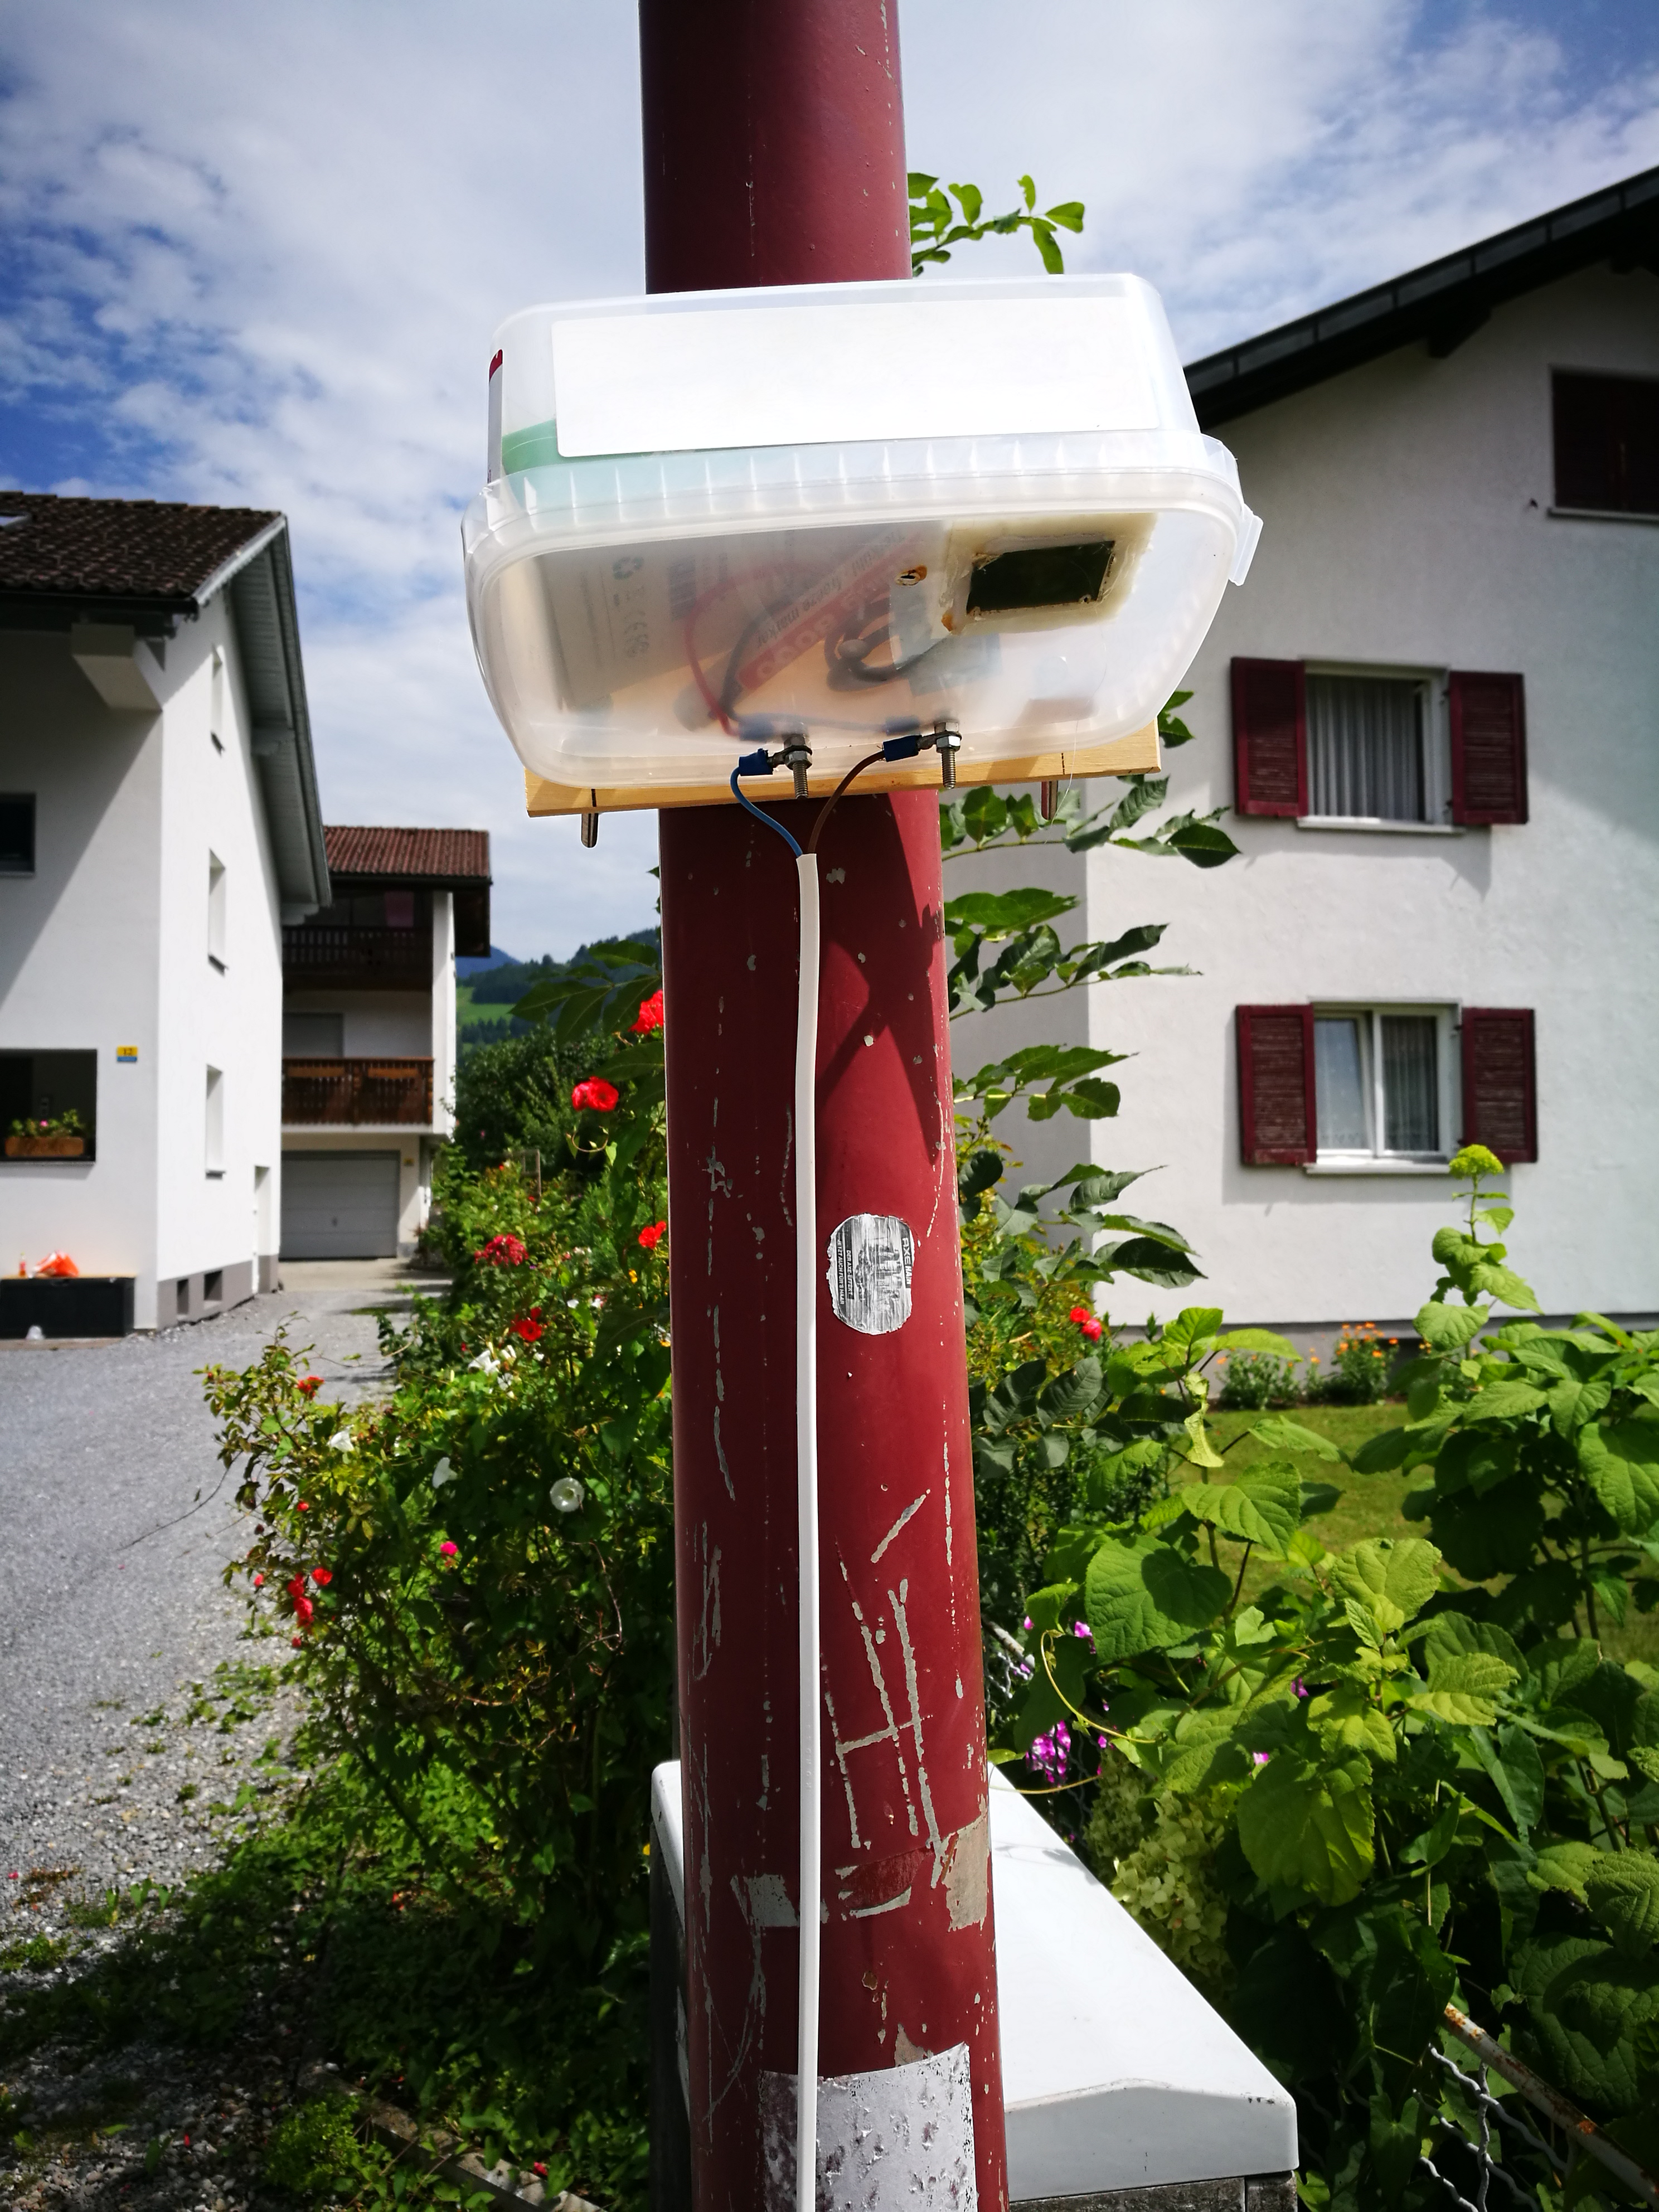
\includegraphics[height=0.6\textwidth]{Hardware/GesamtsystemH.jpg} 
  \caption{Einsatzfähiges Gesamtsystem}
  \label{bGesamtsystemH}
\end{figure}